\section{Red doméstica}

Para este experimento se tomo una captura de 30 minutos de la red Wi-Fi de los labos de la facultad.
\begin{figure}[h]
  \centering
    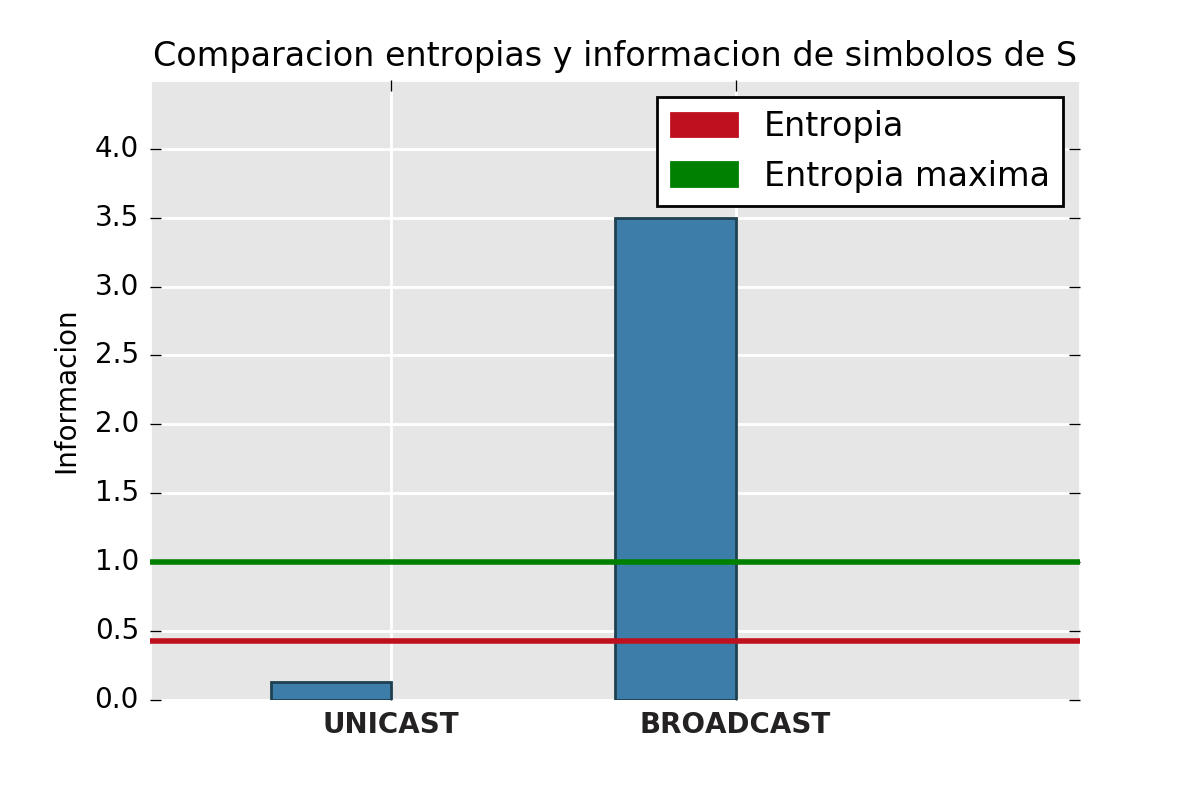
\includegraphics[width=0.45\textwidth]{grafico1-red-labos.png}
  \caption{Entropia de la fuente}
  \label{}
\end{figure}
Como podemos ver en el gráfico comparativo la entropía no llega a ser máxima. 
De hecho puede verse en el símbolo BROADCAST proporciona mucha mas información que el símbolo UNICAST. 
Por lo que hay un mayor flujo de paquetes UNICAST que BROADCAST, "ACA UNA JUSTIFICACION SOBRE LO QUE SUGIERE ESTO ACERCA DE ESTA RED". 

El overhead impuesto por la red influencia la entropia de esta fuente.
Por ejemplo, si hubiese mas mensajes $ARP$ $BROADCAST$ la información del símbolo $S_{BROADCAST}$ 
bajaría haciendo consecuentemente que la entropía de la fuente $S$ se vea modificada.

\begin{figure}[h]
  \centering
    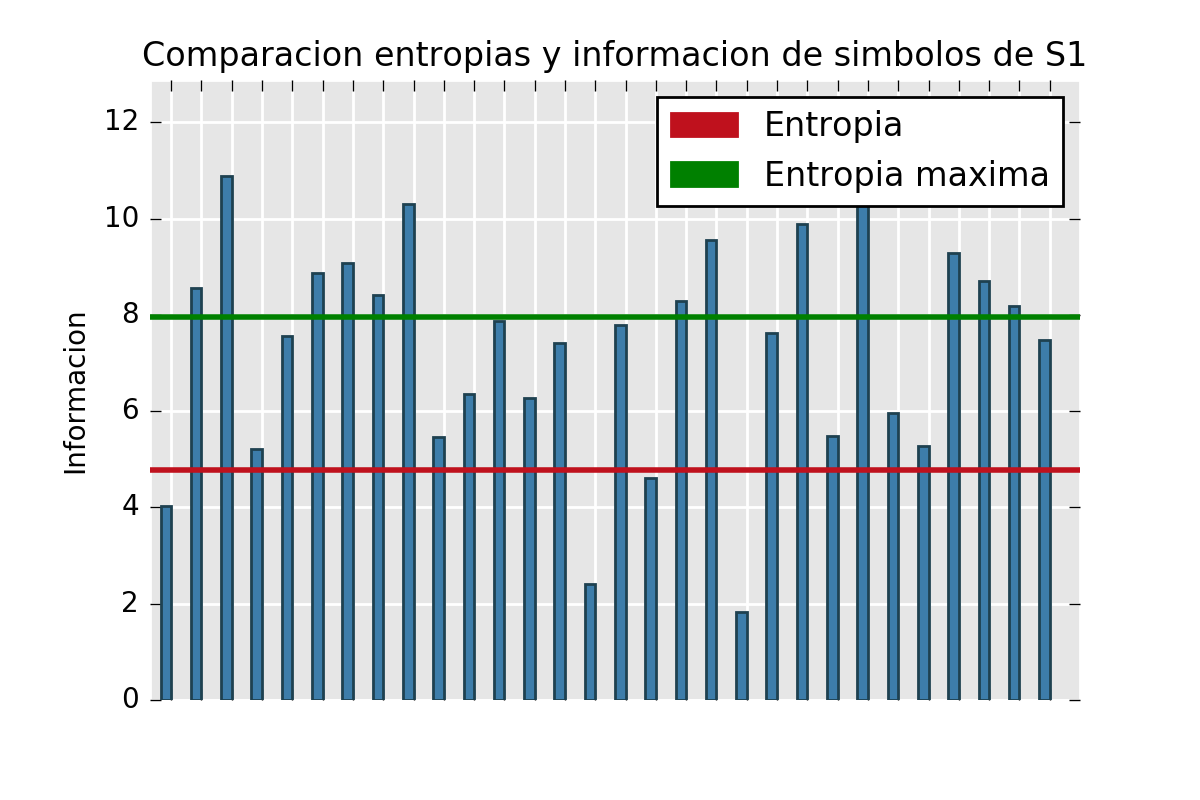
\includegraphics[width=0.45\textwidth]{grafico2-red-labos.png}
  \caption{Entropia de la fuente}
  \label{}
\end{figure}

En comparación con el resto de los mensajes el tráfico $ARP$ es bajo, solo el 4\% de los mensajes son $ARP$. 
En base al criterio propuesto, se pueden distinguir 4 nodos:   

    \begin{table}[ht]\begin{center}
      \begin{tabular}{|c|c|}
      \hline
      \textbf{Nodo} & \textbf{Informacion} \\ \hline
      \texttt{10.2.7.254}& 1.829564 \\ \hline
      \texttt{10.2.203.254}& 2.414527 \\ \hline
      \texttt{10.2.1.250}& 4.026302 \\ \hline
      \texttt{10.2.3.254}& 4.601927 \\ \hline
      \end{tabular}
      \caption{Nodos destacados}
      \label{Nodos-destacados}
    \end{center}\end{table}

Es muy probable que estos nodos distinguidos sean Routers y los dos nodos de menor información podrían ser Default Gateway/s, puesto que como en nuestra fuente estamos tomando las IPs destino de los paquetes $ARP$ $Who-has$. Esto indica que estas IPs son muy frecuentes con lo cual se podria pensar en el escenario en que la mayoría de los nodos quiere conocer la MAC del Default Gateway por lo tanto envían tramas $Who-has$ con la dirección del mismo. 